\section{非微扰 QCD}\label{sec:qcd-nonperturbative-dp15}

前一节的微扰展开以 $g_s(\mathcal Q)$ 为展开参数：每增加一个圈阶，振幅中会多出更高次的耦合。这个组织方式只有在相邻阶通常越来越小时才具有截断意义。当特征物理动量 $\mathcal Q$ 降到 $\Lambda_{\rm QCD}$ 附近时，$\alpha_s(\mathcal Q)$ 达到 $O(1)$，更高圈阶不再天然比低圈阶小；此时继续“多算几圈”不能提供一个由小参数控制的系统逼近。问题不在 QCD 作用量失效，而在以圈数作为近似层级的表示失效。所谓\emph{非微扰 QCD}仍以同一个 QCD 作用量为母定义，但计算方法直接处理完整路径积分、Hamiltonian 谱或规范不变关联函数，而不把有限个 Feynman 圈阶作为主要截断参数。需要计算的物理对象仍然是强子质量、静态源能量、相关函数、热力学量等可观测量；变化的是求解它们的数学表示。

低能区域还允许对 $g_s^2$ 非解析的贡献，例如 $\exp[-8\pi^2/g_s^2]$。这类项在 $g_s=0$ 处没有普通 Taylor 级数，因此有限圈阶不能产生它们。处理这一强耦合区域需要三个彼此衔接的层级：格点路径积分提供保持局域规范对称的紫外调节；Wilson 环、Euclidean 关联函数和 Dirac 谱从中定义静态势、强子谱与凝聚；当外部动量进一步低于强子激发尺度时，低能有效场论只保留轻自由度与对称性。三者共享同一 QCD 对称结构，并通过匹配连接。

\subsection{格点母定义与连续极限}

格点 QCD 首先是一种在有限紫外分辨率下定义路径积分的方法。把实时间作 Wick 旋转 $t=-\ii\tau$ 后，振荡权重 $\exp(\ii S/\hbar)$ 变成欧几里得权重 $\exp(-S_E/\hbar)$；这里 $\tau$ 称为\emph{欧几里得时间}，它是计算变量，不是实验室中的第二种时间。再把连续欧几里得时空替换为间距 $a$ 的超立方格点，$a$ 充当最短可分辨长度，也就是紫外调节器；连续理论对应保持物理量固定后取 $a\to0$ 的极限。为了在有限 $a$ 上仍精确保存局域规范变换，基本变量不直接取格点上的 $\mathscr C_\mu^a$，而取相邻格点之间的平行移动群元素。

欧几里得格点规范理论因此把规范联络改写为沿最短格边的平行移动算符。连续 Wilson 线已经在\eqnrefs{eq:wilson-line-general-dp11} 中定义；采用格点规范理论常用的方向约定，最短链变量为
\begin{equation}
 \boxed{
 U_\mu(x)
 =U_C(x+a\hat\mu,x)^{-1}
 =\exp\!\left[\ii a g_s\mathscr C_\mu(x)+\order(a^2)\right].}
 \label{eq:lattice-link-dp11}
\end{equation}
这里 $U_\mu(x)\in SU(3)$ 是无量纲群元素，$\mathscr C_\mu=\mathscr C_\mu^aT^a$ 是连续规范联络。在格点点变换 $\Omega(x)\in SU(3)$ 下，链变量按两个端点分别变换，因而闭合路径的迹在有限 $a$ 时已经严格规范不变。

四条相邻格边围成的最小闭合正方形称为\emph{格元}（plaquette）。沿这个小回路平行移动一周，得到的群元素测量有限面积上的曲率；它正是连续场强 $\mathcal F_{\mu\nu}$ 的格点版本。最小闭合路径是格元
\begin{equation}
 U_{\mu\nu}(x)
 =U_\mu(x)U_\nu(x+a\hat\mu)
 U_\mu^\dagger(x+a\hat\nu)U_\nu^\dagger(x).
 \label{eq:plaquette-definition-dp11}
\end{equation}
它测量面积 $a^2$ 上的局域曲率。相应的 Wilson 规范作用量写成
\begin{equation}
 \boxed{
 \frac{S_W}{\hbar}
 =\beta_{\rm lat}\sum_{x,\mu<\nu}
 \left[1-\frac1{N_c}\Re\Tr U_{\mu\nu}(x)\right],
 \qquad
 \beta_{\rm lat}=\frac{2N_c}{g_s^2}.}
 \label{eq:wilson-gauge-action-dp11}
\end{equation}
它在 $a\to0$ 时恢复欧几里得 Yang--Mills 作用量
\begin{equation}
 \boxed{
 \frac{S_W}{\hbar}
 \longrightarrow
 \int\dd^4 x\,\frac14\mathcal F_{\mu\nu}^a\mathcal F_{\mu\nu}^a.}
 \label{eq:wilson-continuum-limit-dp11}
\end{equation}
连续极限不是简单地把 $a$ 取成很小：还必须同时控制物理盒长 $L=Na$、轻夸克质量和统计误差。格距外推 $a\to0$ 与无限体积外推 $L\to\infty$ 是彼此独立的系统误差来源。

\begin{figure}[htbp]
\centering
\begin{tikzpicture}[scale=.92,>=Latex,line label/.style={fill=white,fill opacity=.96,text opacity=1,inner sep=1.15pt}]
\foreach \x in {0,1.15,2.3,3.45,4.6}{
  \foreach \y in {0,1.15,2.3,3.45}{\fill (\x,\y) circle (1.15pt);}
}
\foreach \x in {0,1.15,2.3,3.45}{
  \foreach \y in {0,1.15,2.3,3.45}{\draw[thin] (\x,\y)--++(1.15,0);}
}
\foreach \x in {0,1.15,2.3,3.45,4.6}{
  \foreach \y in {0,1.15,2.3}{\draw[thin] (\x,\y)--++(0,1.15);}
}
\draw[line width=1.5pt,->] (1.15,1.15)--(2.3,1.15);
\draw[line width=1.5pt,->] (2.3,1.15)--(2.3,2.3);
\draw[line width=1.5pt,->] (2.3,2.3)--(1.15,2.3);
\draw[line width=1.5pt,->] (1.15,2.3)--(1.15,1.15);
\node[align=left,right] at (4.9,2.75) {link variable $U_\mu(x)$ defined on links};
\node[align=left,right] at (4.9,2.05) {plaquette $U_{\mu\nu}$ measure curvature};
\node[align=left,right] at (4.9,1.35) {$a\to0$ restored as $\mathcal F_{\mu\nu}$};
\end{tikzpicture}
\caption{格点规范理论在调节器层面保持规范不变性。基本自由度是格边上的群元素；闭合格元的完整绕行量在连续极限中给出场强。}
\label{fig:lattice-plaquette-dp11}
\end{figure}

Wick 旋转以后，欧几里得路径积分具有统计平均的形式。这里“统计平均”指对所有允许的规范场组态作加权积分；积分变量是场组态本身，不是实验重复测量得到的一组经典随机轨迹。欧几里得作用量决定每个组态在该数学积分中的权重：
\begin{equation*}
 Z=\int[\dd U]\,\ee^{-S_W[U]/\hbar},
 \qquad
 \langle\mathcal O\rangle
 =\frac1Z\int[\dd U]\,\mathcal O[U]\ee^{-S_W[U]/\hbar}.
\end{equation*}
对纯规范理论，权重实且非负；加入费米子后，Grassmann 积分产生费米子行列式 $\det D_f[U]$，规范场组态因此按海夸克涨落重新加权。这个欧几里得母定义既能给出真空量，也能通过关联函数恢复强子谱。

\subsection{静态势、断弦与有限温度}

Wilson 环是沿闭合路径把规范联络平行移动一周后取颜色迹得到的规范不变量。它可以理解为“一个颜色试探荷绕闭合回路后积累的非阿贝尔相位”。矩形 Wilson 环尤其把这一平行移动与一对静态重颜色源的能量直接联系起来。对空间宽度 $R$、欧几里得时间长度 $T_E$ 的闭合矩形，谱分解为
\begin{equation}
 \langle W(R,T_E)\rangle
 =\sum_n|c_n(R)|^2
 \exp\!\left[-\frac{E_n(R)T_E}{\hbar}\right].
 \label{eq:wilson-loop-spectral-dp11}
\end{equation}
因此长欧几里得时间只保留最低静态能量，定义
\begin{equation}
 \boxed{
 V(R)
 =-\lim_{T_E\to\infty}
 \frac\hbar{T_E}\ln\langle W(R,T_E)\rangle.}
 \label{eq:static-potential-from-wilson-dp11}
\end{equation}
在纯 Yang--Mills 理论中，若大尺度 Wilson 环满足面积律
\begin{equation}
 \langle W(C)\rangle
 \sim\exp\!\left[-\frac{\sigma A(C)}{\hbar c}\right],
 \label{eq:wilson-area-law-dp11}
\end{equation}
则对矩形环 $A=RcT_E$，长欧几里得时间投影给出
\begin{equation}
 \boxed{V(R)=\sigma R+\delta V(R),}
 \label{eq:linear-potential-area-law-dp11}
\end{equation}
其中弦张力 $\sigma$ 的 SI 单位为 J/m。令 $\lambda_{\rm QCD}=\hbar/\Lambda_{\rm QCD}$；面积律描述的红外区域要求 $R/\lambda_{\rm QCD}\gg1$，而有限 $T_E$ 的激发态污染按 $\exp[-(E_1-E_0)T_E/\hbar]$ 抑制。$\delta V$ 收集周长自能、有限尺寸及其他次领长程项，因此线性势是大环渐近首项而非任意 $R$ 上的恒等式。完整 QCD 含动力学轻夸克时，足够长的色通量管可以产生轻夸克对并发生断弦；纯规范面积律因而是最清楚的禁闭判据，而真实 QCD 的低能谱还必须同时考虑动力学物质场。

有限温度把欧几里得时间压缩到 $\beta_T\hbar=\hbar/(k_BT)$。沿整个欧几里得时间圆周的 Polyakov 线
\begin{equation*}
 L(\mathbf x)
 =\frac1{N_c}\Tr\,\mathcal P
 \exp\!\left[
 \ii g_s\int_0^{\beta_T\hbar}\dd\tau\,
 \mathscr C_0(\tau,\mathbf x)
 \right]
\end{equation*}
测量放入一个静态基本表示色源的自由能。纯 Yang--Mills 理论中，中心对称性使 $\langle L\rangle$ 成为退禁闭相变的序参量；动力学夸克显式破坏中心对称性，因此真实 QCD 中通常讨论有限温度交叉过渡，而不能把 $\langle L\rangle=0$ 当作唯一的禁闭定义。

\subsection{拓扑扇区与瞬子}

欧几里得 Yang--Mills 场按整数 Pontryagin 数 $Q_{\rm top}$ 分成彼此不能通过有限作用量小变形连续连接的拓扑扇区。场强与其对偶之间的平方完成给出
\begin{equation}
 \boxed{
 \frac{S_E}{\hbar}
 \ge\frac{8\pi^2}{g_s^2}|Q_{\rm top}|.}
 \label{eq:instanton-action-bound-dp11}
\end{equation}
等号由自对偶或反自对偶场强达到。$|Q_{\rm top}|=1$ 的半经典鞍点因而带有 $\exp[-8\pi^2/g_s^2]$ 权重，明确显示出非微扰的非解析耦合依赖。拓扑扇区进一步通过轴反常与 $\theta$ 角进入强 CP 问题；这里的作用量下界只说明半经典拓扑鞍点的尺度，并不把瞬子解释成普通渐近粒子。

\subsection{Dirac 谱、手征凝聚与低能自由度}

质量趋于零时，$N_f$ 个轻味的经典 QCD 拉格朗日量具有
\begin{equation*}
 SU(N_f)_L\times SU(N_f)_R
\end{equation*}
的非单态手征对称性。若真空形成非零凝聚 $\langle\bar\psi\psi\rangle$，许多彼此由这个连续对称变换连接的真空具有相同能量；沿这些等能真空的切向方向移动没有恢复力。Goldstone 定理表明：每个被真空选择破坏的连续生成元都对应一个低能无隙模。对 $SU(N_f)_L\times SU(N_f)_R\to SU(N_f)_V$，这样的方向共有 $N_f^2-1$ 个。

现实中的轻夸克质量虽小却不为零，它给这些平坦方向一个很弱的恢复力，于是无隙模获得小质量，称为赝 Goldstone 玻色子。两轻味情形恰有三个这样的模，即三种 \(\pi\) 介子。味单态轴变换 $U(1)_A$ 不属于这组低能模：它已经被量子反常显式破坏，所以不会再多产生一个轻粒子。这样，只需回答两个定量问题：凝聚怎样从 QCD 本身读出，以及小夸克质量怎样把这些低能模抬到有限质量。

手征凝聚可以直接由欧几里得 Dirac 算符在零本征值附近的谱密度读取。令
\begin{equation}
 \slashed D_E\phi_n=\ii\lambda_n\phi_n,
 \qquad \lambda_n\in\mathbb R,
 \qquad
 \rho(\lambda)\equiv\lim_{V_4\to\infty}\frac1{V_4}\sum_n\delta(\lambda-\lambda_n).
 \label{eq:qcd-dirac-spectral-density-dp68}
\end{equation}
并以四维体积归一化定义全谱密度 $\rho(\lambda)$。先取热力学极限，再取轻夸克质量 $m\to0^+$，得到 Banks--Casher 关系
\begin{equation}
 \boxed{
 -\langle\bar\psi\psi\rangle_{\text{每个轻味}}
 =\pi\rho(0).}
 \label{eq:banks-casher-dp11}
\end{equation}
因此自发手征对称性破缺可以等价地表述为：热力学极限下 Dirac 本征值在零点附近保持有限谱密度。这里两个极限的顺序不可交换；有限体积中的离散谱本身不能产生严格的自发对称性破缺。

凝聚给出了低能有效自由度的对称性来源。以两轻味为例，把三个 \(\pi\) 介子组织到无量纲矩阵场
\begin{equation*}
 U(x)=\exp\!\left[\frac{\ii\,\pi^a(x)\tau^a}{F_\pi}\right]\in SU(2),
\end{equation*}
其中 $F_\pi$ 采用能量归一化，$\pi^a$ 也具有能量量纲。对外部四动量 $p$ 和 \(\pi\) 介子质量满足
\begin{equation}
 \boxed{
 \epsilon_\chi
 =\frac{\max(pc,m_\pi c^2)}{4\pi F_\pi}\ll1}
 \label{eq:qcd-chiral-control-dp33}
\end{equation}
时，最低阶手征有效作用量只允许两个独立结构：Goldstone 场的两导数动能项，以及由轻夸克质量矩阵 $M_q=\operatorname{diag}(m_uc^2,m_dc^2)$ 引起的显式破缺项。把 $B_0$ 定义为把轻夸克质量能量映射成赝 Goldstone 质量平方的低能常数，领先作用量写成
\begin{equation}
 \boxed{
 \frac{S_\chi}{\hbar}
 =\int\dd^4 x\left[
 \frac{F_\pi^2}{4(\hbar c)^2}
 \Tr(\partial_\mu U^\dagger\partial^\mu U)
 +\frac{F_\pi^2B_0}{2(\hbar c)^4}
 \Tr\!\left(M_qU^\dagger+UM_q\right)
 \right]+\cdots .}
 \label{eq:qcd-chiral-lo-action-dp33}
\end{equation}
省略项至少多含两个导数、一个额外轻夸克质量插入，或一个圈因子。把\eqnrefs{eq:qcd-chiral-lo-action-dp33} 展开到 \(\pi\) 介子场二次阶，得到 Gell--Mann--Oakes--Renner 关系
\begin{equation}
 \boxed{
 m_\pi^2c^4F_\pi^2
 =-(m_u+m_d)c^2(\hbar c)^3
 \langle\bar q q\rangle
 +\order(m_q^2).}
 \label{eq:qcd-gmor-dp33}
\end{equation}
这里 $\langle\bar q q\rangle$ 表示两轻味在同位旋极限中的单味凝聚，并采用约定 $B_0=-(\hbar c)^3\langle\bar q q\rangle/F_\pi^2$。因此 Banks--Casher 关系给出的零模谱密度并不只说明“真空有序”：它还通过 $B_0$ 控制 \(\pi\) 介子质量对显式轻夸克质量的领先响应。

格点计算最终需要从欧几里得关联函数恢复强子能谱。对具有目标量子数的插值算符 $\mathcal O$，零空间动量两点函数为
\begin{equation}
 \boxed{
 C_{\mathcal O}(\tau)
 =\int\dd^3 \mathbf x\,
 \langle\mathcal O(\tau,\mathbf x)\mathcal O^\dagger(0)\rangle
 =\sum_n |Z_n|^2\ee^{-E_n\tau/\hbar},
 \qquad \tau>0.}
 \label{eq:qcd-euclidean-correlator-spectrum-dp31}
\end{equation}
其中 $E_n$ 是该量子数扇区的能量，$Z_n$ 是插值算符与第 $n$ 个态的重叠。若最低态与第一激发态之间存在可分辨谱隙，则离散时间步长 $\Delta\tau$ 定义的有效能量
\begin{equation}
 \boxed{
 E_{\rm eff}(\tau)
 =-\frac{\hbar}{\Delta\tau}
 \ln\frac{C_{\mathcal O}(\tau+\Delta\tau)}{C_{\mathcal O}(\tau)}
 \longrightarrow E_0}
 \label{eq:qcd-euclidean-effective-energy-dp31}
\end{equation}
在足够大的 $\tau$ 上出现平台。平台过早拟合会受到激发态污染，过晚又会遭受指数恶化的统计信噪比；强子谱提取因此本质上是一个受谱隙、算符重叠和统计噪声共同控制的反问题。

单个插值算符通常只能稳定给出最低态。为了同时分辨若干低激发态，取一组具有相同守恒量子数但空间结构不同的插值算符 $\{\mathcal O_i\}$，构造相关矩阵
\begin{equation}
 C_{ij}(\tau)=\langle\mathcal O_i(\tau)\mathcal O_j^\dagger(0)\rangle
 =\sum_n Z_i^{(n)}Z_j^{(n)*}\ee^{-E_n\tau/\hbar}.
 \label{eq:qcd-correlator-matrix-spectrum-dp68}
\end{equation}
在参考时间 $\tau_0$ 上求解广义本征值问题
\begin{equation}
 \boxed{
 C(\tau)\,v_n(\tau,\tau_0)
 =\lambda_n(\tau,\tau_0)\,C(\tau_0)\,v_n(\tau,\tau_0),
 \qquad
 \lambda_n\sim
 \exp\!\left[-\frac{E_n(\tau-\tau_0)}{\hbar}\right].}
 \label{eq:qcd-gevp-spectrum-dp32}
\end{equation}
这就是格点谱学常用的变分接口：本征向量选择算符空间中与第 $n$ 个能量本征态重叠最大的方向，本征值的长时间指数斜率给出 $E_n$。可靠的激发态谱要求算符基足以覆盖目标态、$C(\tau_0)$ 在保留子空间内条件良好，并且拟合窗口同时避开短时间高激发态污染与长时间统计噪声。

\begin{figure}[htbp]
 \centering
 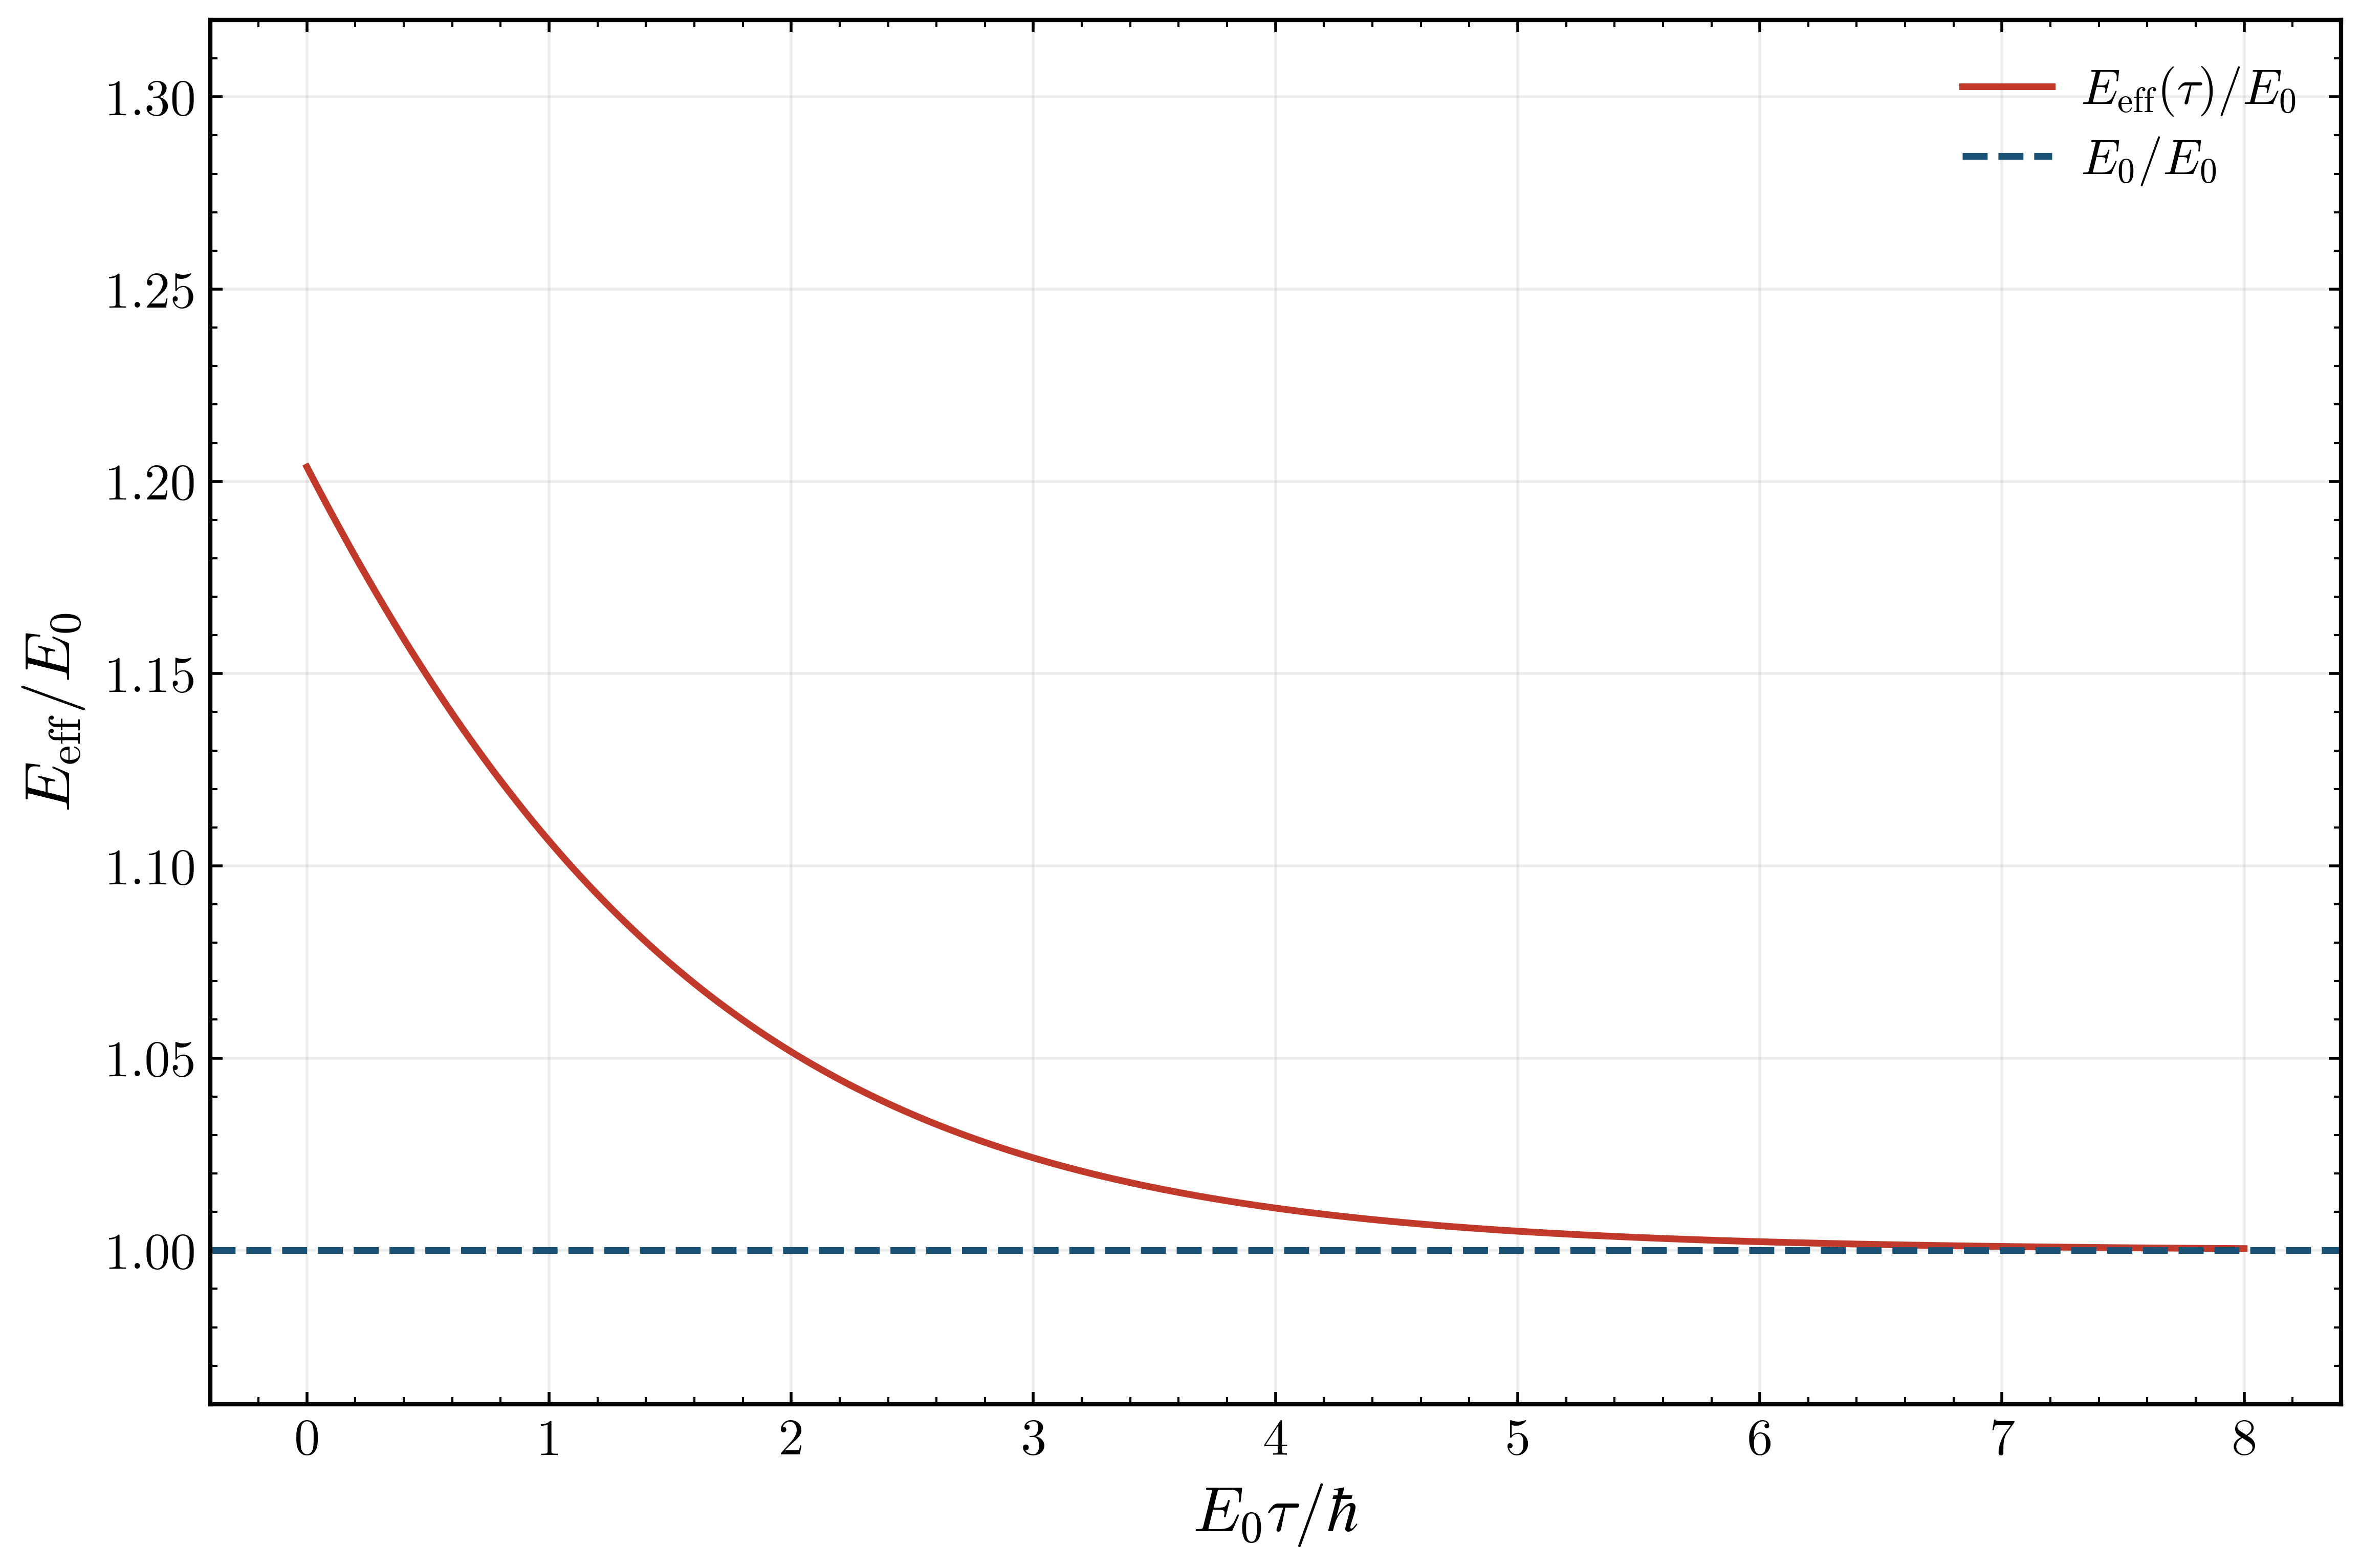
\includegraphics[width=.78\linewidth]{content/FreeElectronQuantumOptics/figures/generated/qcd_euclidean_effective_energy_dp31.png}
 \caption{两态欧几里得关联函数的有效能量示意。横轴和纵轴均按基态能量 $E_0$ 无量纲化；较小 $\tau$ 区域含明显激发态污染，而 $E_{\rm eff}/E_0\to1$ 的平台给出基态能量。曲线由\eqnrefs{eq:qcd-euclidean-effective-energy-dp31} 直接计算。}
 \label{fig:qcd-euclidean-effective-energy-dp31}
\end{figure}

高能 QCD 用重整化微扰理论、重整化群和因子化组织可计算展开；低能区则回到规范不变的欧几里得路径积分。链变量与格元给出保持规范不变性的调节器，Wilson 环给出静态势，拓扑扇区给出非解析半经典结构，Dirac 谱给出手征凝聚，领先手征有效作用量把凝聚连接到轻介子谱，欧几里得关联函数再把这些母定义连接到实际强子能级。禁闭、手征对称性破缺和拓扑效应彼此相关，但没有任何一个能够由“一圈耦合变大”单独推出。


\begin{derivation}[从\eqnrefs{eq:wilson-gauge-action-dp11}到\eqnrefs{eq:wilson-continuum-limit-dp11}]
由小闭合路径与曲率的关系，格元满足

\begin{equation*}
 U_{\mu\nu}(x)
 =\exp\!\left[\ii g_sa^2\mathcal F_{\mu\nu}(x)+\order(a^3)\right].
\end{equation*}
展开指数并使用 $\Tr T^a=0$ 与 $\Tr(T^aT^b)=\delta^{ab}/2$，有
\begin{align*}
 \Re\Tr U_{\mu\nu}
 &=N_c-
 \frac{g_s^2a^4}{2}
 \Tr\!\left(\mathcal F_{\mu\nu}\mathcal F_{\mu\nu}\right)
 +\order(a^6),\\
 &=N_c-
 \frac{g_s^2a^4}{4}
 \mathcal F_{\mu\nu}^a\mathcal F_{\mu\nu}^a
 +\order(a^6).
\end{align*}
代入\eqnrefs{eq:wilson-gauge-action-dp11}，并用 $\beta_{\rm lat}=2N_c/g_s^2$，得到
\begin{equation*}
 \frac{S_W}{\hbar}
 =\sum_xa^4\sum_{\mu<\nu}
 \frac12\mathcal F_{\mu\nu}^a\mathcal F_{\mu\nu}^a
 +\order(a^2).
\end{equation*}
反对称性给
\begin{equation*}
 \sum_{\mu<\nu}\mathcal F_{\mu\nu}^2
 =\frac12\sum_{\mu,\nu}\mathcal F_{\mu\nu}^2,
\end{equation*}
而 Riemann 和在 $a\to0$ 时变成四维积分，因此得到相应的欧几里得 Yang--Mills 连续极限。
\end{derivation}



\begin{derivation}[从\eqnrefs{eq:pontryagin-number-dp11}到\eqnrefs{eq:instanton-action-bound-dp11}]
在四维欧几里得空间定义
\[
({}^\star\!\mathcal F)_{\mu\nu}^a
\equiv\frac12\epsilon_{\mu\nu\rho\sigma}
\mathcal F_{\rho\sigma}^a.
\]
欧几里得号差使 $({}^\star)^2=+1$ 作用在二形式上，并且
\[
({}^\star\!\mathcal F)_{\mu\nu}^a
({}^\star\!\mathcal F)_{\mu\nu}^a
=\mathcal F_{\mu\nu}^a\mathcal F_{\mu\nu}^a.
\]
因此对任一符号都有非负平方
\begin{align*}
0
&\le\frac12\int\dd^4x\,
\bigl(\mathcal F_{\mu\nu}^a
\mp{}^\star\!\mathcal F_{\mu\nu}^a\bigr)^2\\
&=\int\dd^4x\,
\mathcal F_{\mu\nu}^a\mathcal F_{\mu\nu}^a
\mp\int\dd^4x\,
\mathcal F_{\mu\nu}^a{}^\star\!\mathcal F_{\mu\nu}^a.
\end{align*}
选择使第二项与拓扑积分同号的那个符号，便得到
\[
\int\dd^4x\,
\mathcal F_{\mu\nu}^a\mathcal F_{\mu\nu}^a
\ge
\left|
\int\dd^4x\,
\mathcal F_{\mu\nu}^a{}^\star\!\mathcal F_{\mu\nu}^a
\right|.
\]
正文\eqnrefs{eq:pontryagin-number-dp11} 的归一化是
\[
Q_{\rm top}
=\frac{g_s^2}{32\pi^2}
\int\dd^4x\,
\mathcal F_{\mu\nu}^a{}^\star\!\mathcal F_{\mu\nu}^a,
\]
相应的欧几里得 Yang--Mills 作用量为
\[
\frac{S_E}{\hbar}
=\frac14\int\dd^4x\,
\mathcal F_{\mu\nu}^a\mathcal F_{\mu\nu}^a.
\]
两式代入上界，严格得到
\[
\boxed{
\frac{S_E}{\hbar}
\ge\frac{8\pi^2}{g_s^2}|Q_{\rm top}|.}
\]

等号何时成立也不是另加条件：非负平方的积分只有在平方逐点为零时才能饱和，因此
\[
\mathcal F_{\mu\nu}^a
=\pm{}^\star\!\mathcal F_{\mu\nu}^a.
\]
这就是自对偶/反自对偶方程。对 $|Q_{\rm top}|=1$，饱和作用量为 $8\pi^2\hbar/g_s^2$，半经典路径积分权重因而含
\[
\exp\!\left(-\frac{S_E}{\hbar}\right)
=\exp\!\left(-\frac{8\pi^2}{g_s^2}\right),
\]
它在 $g_s=0$ 处具有本质奇点，不能由有限阶耦合常数幂级数产生；这就是“瞬子效应是非微扰的”在数学上的具体含义。
\end{derivation}

\begin{derivation}[从\eqnrefs{eq:qcd-dirac-spectral-density-dp68}到\eqnrefs{eq:banks-casher-dp11}]
正文采用欧几里得 Dirac 算符的反厄米 convention
\begin{equation*}
 \slashed D_E\phi_n=\ii\lambda_n\phi_n,
 \qquad \lambda_n\in\mathbb R,
 \qquad
 \int_{V_4}\dd^4 x\,\phi_m^\dagger\phi_n=\delta_{mn}.
\end{equation*}
无质量算符与 $\gamma^5$ 反对易：
\begin{equation*}
 \{\gamma^5,\slashed D_E\}=0.
\end{equation*}
因此若 $\lambda_n\neq0$，则
\begin{equation*}
 \slashed D_E(\gamma^5\phi_n)
 =-\ii\lambda_n(\gamma^5\phi_n),
\end{equation*}
非零谱严格成 $\pm\lambda$ 对。加入小而正的夸克质量，欧几里得传播子为
\begin{equation*}
 S_E=(\slashed D_E+mc/\hbar)^{-1},
\end{equation*}
因此单味凝聚由 coincident propagator 的迹给出
\begin{equation*}
 -\langle\bar\psi\psi\rangle_m
 =\frac1{V_4}
 \left\langle\Tr\frac1{\slashed D_E+mc/\hbar}\right\rangle.
\end{equation*}
在 $\phi_n$ 本征基中插入完备关系：
\begin{equation*}
 \Tr\frac1{\slashed D_E+mc/\hbar}
 =\sum_n\frac1{\ii\lambda_n+mc/\hbar}.
\end{equation*}
对每一对非零本征值 $\pm\lambda$，
\begin{align*}
 \frac1{\ii\lambda+mc/\hbar}
 +\frac1{-\ii\lambda+mc/\hbar}
 &=\frac{2mc/\hbar}{\lambda^2+(mc/\hbar)^2}.
\end{align*}
于是
\begin{equation*}
 -\langle\bar\psi\psi\rangle_m
 =\frac1{V_4}\left\langle
 \frac{N_0}{mc/\hbar}
 +\sum_{\lambda_n>0}
 \frac{2mc/\hbar}{\lambda_n^2+(mc/\hbar)^2}
 \right\rangle,
\end{equation*}
其中 $N_0$ 是严格零模数。固定拓扑荷时 $N_0=O(1)$，故先取 $V_4\to\infty$ 后 $N_0/V_4\to0$；自发凝聚来自零点附近数目随体积成比例增长的近零模，而不是有限个拓扑零模。

按正文\eqnrefs{eq:qcd-dirac-spectral-density-dp68}，热力学极限把全谱离散求和变成
\begin{equation*}
 \lim_{V_4\to\infty}
 \frac1{V_4}\left\langle\sum_n f(\lambda_n)\right\rangle
 =\int_{-\infty}^{+\infty}\dd\lambda\,\rho(\lambda)f(\lambda).
\end{equation*}
由于 $\rho(-\lambda)=\rho(\lambda)$，传播子迹中的奇函数部分积分为零，只剩
\begin{equation*}
 -\langle\bar\psi\psi\rangle_m
 =\int_{-\infty}^{+\infty}\dd\lambda\,
 \rho(\lambda)
 \frac{mc/\hbar}{\lambda^2+(mc/\hbar)^2}.
\end{equation*}
令 $\epsilon=mc/\hbar$。对任意在零点连续的谱密度，分布极限
\begin{equation*}
 \lim_{\epsilon\to0^+}
 \frac{\epsilon}{\lambda^2+\epsilon^2}
 =\pi\delta(\lambda)
\end{equation*}
直接给出
\begin{align*}
 -\lim_{m\to0^+}\lim_{V_4\to\infty}
 \langle\bar\psi\psi\rangle_m
 &=\pi\int_{-\infty}^{+\infty}\dd\lambda\,
 \rho(\lambda)\delta(\lambda)\\
 &=\pi\rho(0),
\end{align*}
即正文\eqnrefs{eq:banks-casher-dp11}。若有 $N_f$ 个简并轻味，则每个味都满足同一关系，而味求和的凝聚相应多出因子 $N_f$。若把极限顺序反过来，有限体积谱仍是离散的，除有限个拓扑零模外没有连续的零点谱密度；因此 $V_4\to\infty$ 必须先于 $m\to0^+$，这正是自发对称性破缺所需的热力学极限。
\end{derivation}

\begin{derivation}[从\eqnrefs{eq:qcd-chiral-lo-action-dp33}到\eqnrefs{eq:qcd-gmor-dp33}]
取两轻味同位旋极限，并把

\begin{equation*}
 U=\exp\!\left(\frac{\ii\pi}{F_\pi}\right),
 \qquad
 \pi=\pi^a\tau^a,
 \qquad
 \Tr(\tau^a\tau^b)=2\delta^{ab}.
\end{equation*}
展开到二次阶，
\begin{align*}
 U&=1+\frac{\ii\pi}{F_\pi}-\frac{\pi^2}{2F_\pi^2}+\order(\pi^3),\\
 U^\dagger&=1-\frac{\ii\pi}{F_\pi}-\frac{\pi^2}{2F_\pi^2}+\order(\pi^3).
\end{align*}
动能项因而变成
\begin{align*}
 \frac{F_\pi^2}{4(\hbar c)^2}
 \Tr(\partial_\mu U^\dagger\partial^\mu U)
 &=\frac1{4(\hbar c)^2}
 \Tr(\partial_\mu\pi\,\partial^\mu\pi)+\order(\pi^4),\\
 &=\frac1{2(\hbar c)^2}
 \partial_\mu\pi^a\partial^\mu\pi^a+\order(\pi^4),
\end{align*}
得到三个规范归一化的实标量低能模。

质量矩阵在同位旋极限中为 $M_q=\hat m c^2 I_2$，其中 $\hat m=(m_u+m_d)/2$。线性 \(\pi\) 介子项在 $U+U^\dagger$ 中相消，而二次项给
\begin{align*}
 \Tr[M_q(U^\dagger+U)]
 &=4\hat m c^2
 -\frac{\hat m c^2}{F_\pi^2}\Tr(\pi^2)+\order(\pi^4),\\
 &=4\hat m c^2
 -\frac{2\hat m c^2}{F_\pi^2}\pi^a\pi^a+\order(\pi^4).
\end{align*}
代回\eqnrefs{eq:qcd-chiral-lo-action-dp33}，二次质量项为
\begin{equation*}
 -\frac{B_0\hat m c^2}{(\hbar c)^4}\pi^a\pi^a.
\end{equation*}
与标准二次作用量中的
\begin{equation*}
 -\frac{m_\pi^2c^4}{2(\hbar c)^4}\pi^a\pi^a
\end{equation*}
比较，得到
\begin{equation*}
 m_\pi^2c^4=2B_0\hat m c^2=B_0(m_u+m_d)c^2.
\end{equation*}
最后使用已定义的低能常数匹配
\begin{equation*}
 B_0=-\frac{(\hbar c)^3\langle\bar q q\rangle}{F_\pi^2},
\end{equation*}
即可得到\eqnrefs{eq:qcd-gmor-dp33}。该关系的修正由更高阶轻夸克质量插入与手征圈图共同控制，其相对大小按\eqnrefs{eq:qcd-chiral-control-dp33} 的幂次计数组织。
\end{derivation}

